\sys dynamically {\em coalesces} consecutively executing tasks at run time. When two tasks are coalesced, the first of the two tasks does not commit its updates to protected memory locations when it reaches a \transition statement. Instead, execution immediately continues from the beginning of the second of the two tasks. At the end of the second of the two coalesced tasks, \sys commits the pages that were updated by either of the coalescing tasks. The purpose of coalescing is to better amortize the run time overhead of committing updated pages when a task ends. If consecutive tasks access the same pages of data, the pages accessed by both tasks only need to be committed once.  

\sys can coalesce an arbitrary number of consecutive tasks. As more tasks coalesce, their collective commit overhead amortizes better, potentially improving performance. As more tasks coalesce, the amount of potentially {\em wasted work} also increases. If power fails during a long sequence of coalesced tasks the lack of an intervening commit requires execution to restart from the {\em first} task in the sequence, failing to preserve the progress of any of the tasks in the long sequence. \sys moderates the risk of coalescing and capitalizes on its benefit by dynamically, \emph{adaptively} determining a coalescing factor that combines many tasks without suffering an excess of wasted work. 

The challenge to coalescing tasks is determining how many tasks to coalesce before committing. During execution, an executing task is either a {\em coalesced} task, which does not commit its state before transitioning or a {\em committing} task, which does commit its state before transitioning. \sys monitors a program's execution to adaptively determine $C$, the number of tasks to coalesce before committing; \sys repeatedly executes $C-1$ coalesced tasks, followed by a committing task. 

\sys determines $C$ for a given operation based on the number of tasks completed, $S$, during the last operational period. \sys begins execution in a coalesced task with an infinite $C$ value. With a continuous power supply, the system executes from the start with all tasks as coalesced tasks entirely avoiding the cost of committing state. On intermittent power, the system executes a sequence of tasks that is interrupted by a power failure. \sys explicitly tracks $S$ during the previous operating period. \sys assigns $C$ to be equal to half of the value of $S$. If more tasks in total are able to complete in an operating period, \sys attempts to coalesce more tasks during the next operating period. If fewer tasks complete, \sys attempts to coalesce fewer tasks during the next operating period. $S$ includes the count of both coalesced and committing tasks completed. If no committing task completes, i.e., execution does not make progress, \sys updates $S$ and attempts to coalesce fewer tasks during the next operating period.

\begin{figure}
	\centering
	\subfloat[Core of task coalescing: commit postponing]{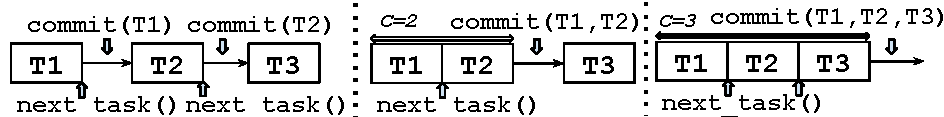
\includegraphics[width=\columnwidth]{figures/coalescing_states}\label{fig:coalescing_example_states}}\\
	\subfloat[Adaptive task coalescing based on task failure history]{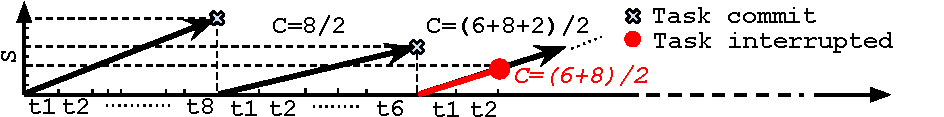
\includegraphics[width=\columnwidth]{figures/coalescing_flowchart}\label{fig:coalescing_example_flowchart}}
	\caption{\sys task coalescing process.}
	\label{fig:coalescing_example}
\end{figure}

\noindent\textbf{Task Coalescing Illustration:} Figure~\ref{fig:coalescing_example_states} (left) shows a sequence of three tasks executing in \sys with no coalescing, incurring the cost of commit at each task transition. The same figure shows the same sequence of tasks executing as coalesced groups of three tasks $C=2$ (center) and $C=3$ (right). Figure~\ref{fig:coalescing_example_flowchart} shows how \sys adapts the value of $C$ based on $S$. \sys executes tasks in the first operating period, assigning the \emph{half of sum of all previous $S$ periods} (in the example case: $C=8/2$). \sys completes then coalesced tasks successfully (four tasks were executed) and in the next operating period, i.e. $C=(8+4)/2$. In the third task execution, power fails after the second task. Then \sys re-executes coalesced task since the previous failure and sets $C=(6+8+2)/2$ in the next operating period. If a larger number of tasks successfully complete in the next operating period, i.e., $S$ is larger, $C$ correspondingly increases, allowing more aggressive coalescing.

%However, it takes a conservative approach by making the virtual task size equal
%to the half of the number of successfully executed real tasks before the last
%power interrupt (see lines~\ref{algo:coalescing:executionHistory1},
%\ref{algo:coalescing:executionHistory2} of Algorithm~\ref{algo:coalescing}). 
%
%We
%advocate for the algorithm conservative approach by the following two reasons:
%(i) the power interrupts are not uniformly distributed over the tasks; and (ii)
%the re-execution penalty, in case of a power interrupt, grows linearly with the
%size of a virtual task. 
%
%Furthermore, the algorithm considers the charging rate
%by allowing the real tasks counter (RTC), which represents the execution
%history between the last two power interrupts, to increase from one up to
%multiple virtual tasks (see line~\ref{algo:coalescing:realTaskCounter} of
%Algorithm~\ref{algo:coalescing}). 
%
%As a consequence, the virtual task size
%changes rapidly (since it is half of the execution history) in response to the
%change in the charging rate. 
%
%However, the algorithm sets a limit to the size of
%the virtual task for these two reasons: (i) having an infinity virtual task
%size, results in a certain computation progress loss; and (ii) the benefit of
%task merging is governed by the diminishing return principle (which will be
%demonstrated experimentally in Section~\ref{sec:results_coalescing}).
%
%The algorithm protects itself from power interrupts by going into three stages:
%(i) virtual progressing, where the operations are done on the volatile memory
%(see
%lines~\ref{algo:coalescing:virtualProgressing1}--\ref{algo:coalescing:virtualProgressing2}
%of Algorithm~\ref{algo:coalescing} ); 
%(ii) transition stage, where the volatile
%state is moved to a temporary persistent buffer. 
%
%Until the end of the second
%stage if a power is interrupted, then all the virtual progress will be
%cancelled and the virtual task will re-executed and re-initialized from a
%consistent input (see line~\ref{algo:coalescing:virtualProgressing1} of
%Algorithm~\ref{algo:coalescing}); 
%
%and (iii) persistent commit stage, upon
%entering this stage the algorithm will make a firm transition (see
%lines~\ref{algo:coalescing:firmTransition1},
%\ref{algo:coalescing:firmTransition2} of Algorithm~\ref{algo:coalescing}) and
%it will not go back to the other stages unless all the data is committed from
%the persistent buffer to non-volatile memory. 
%
%Since the data is being moved in one direction and from a persistent location,
%power interrupt is tolerable at this stage. 

%\begin{algorithm}[t]
%	\caption{\sys task coalescing mechanism}
%	\label{algo:coalescing}
%	\scriptsize
%	\begin{algorithmic}[1]
%		\State $\text{p}$  \Comment{Indicates persistent variables, initialized \textbf{only} during device programming}
%		\State $\text{RT} \in \{\sys~\text{static tasks}\}$  \Comment{Real task}
%		\State $\text{VT} \subset \{~\text{RT's}\}$  \Comment{Virtual task}
%		\State $\text{RTC}$  \Comment{RT counter}
%		\State $\text{VTC}$  \Comment{VT counter}
%		% \State $|\text{VT}|$ \Comment{VT size measured in RT}
%		\State $\text{TVT}$ \Comment{Temporary VT}
%		\State $\text{VT}_{\max}$ \Comment{Maximum VT size measured in RT (coalescing upper bound)}
%		\vspace{0.1cm}
%		
%		\State $\text{p RTC} = x $ 
%		\State $\text{p VT}_{\max} = y$
%		\State $\text{p VT} = \text{RT}$ 
%		\State $\text{p TVT} = \text{VT} $ 
%		\State $\text{VTC} = 0 $ 
%		\vspace{0.1cm}
%
%		\Function{scheduler}{\null}
%
%			\State $\text{VTC} = \text{RTC/2} $  \label{algo:coalescing:executionHistory1}
%			\State $\text{RTC} = 0 $
%			\State $\text{RT} = \text{VT}$ \Comment{Recover virtual state} \label{algo:coalescing:virtualProgressing1}
%			\If{commiting}
%				\State $\text{RT}=\text{TVT}$
%				\State $\texttt{goto} \ \ \ref{commitStage}$ \label{algo:coalescing:firmTransition1}
%			\EndIf
%			\vspace{0.1cm}
%
%			\While {True}
%				\While{$\text{VTC}--$}
%					\Function{execute}{$\text{RT}$}
%					\EndFunction
%					\If{$\text{RTC} < \text{VT}_{\max}$}
%						\State $\text{RTC}++$  \label{algo:coalescing:realTaskCounter}
%					\EndIf
%					\State $\text{RT} \leftarrow \text{RT}_{next}$ \Comment{Virtual progressing}
%				\EndWhile        \label{algo:coalescing:virtualProgressing2}
%
%				\State \Comment{Virtual task is finished}
%				\State $\text{Data} \rightarrow \text{pTempBuf}$ \Comment{pTempBuf: persistent temporary buffer}
%				\State $\text{TVT} = \text{RT}$ 
%				\State $\text{commiting} = \text{True}$ \label{algo:coalescing:firmTransition2}
%				\State 
%				\State $\text{VT} = \text{TVT}$ \label{commitStage}
%				\State $\text{pTempBuf} \rightarrow \text{FRAM}$ 
%				\State $\text{VTC} = \text{RTC/2}$ 		\Comment{Set VT size} \label{algo:coalescing:executionHistory2}
%				\State $\text{commiting} = \text{False}$ 
%
%			\EndWhile
%
%		\EndFunction
%			
%	\end{algorithmic}
%\end{algorithm}

%\subsection{Power Interrupt Immune Scheduler}
%
%% TNT :  Total Number of Tasks
% JT 	: Total Jump
% ID	: Task ID
% D	: relative Jump (Delta)
% VCT_PT : Current Task Pointer

% if(TJ < TNT)
% 	VCT_PT <- VCT_PT + D
% else
% 	while ((dis = TJ - TNT) > TNT)
% 		dis -= ID
% 	VCT_PT <- VCT_PT + dis


\begin{algorithm}[t]
	\caption{\sys's scheduler: relative jump algorithm}
	\label{algo:relativeJump}
	\scriptsize
	%\small
	\begin{algorithmic}[1]
			\State \textsf{TNT}: Total Number of Tasks
			\State \textsf{ID}: Task ID
			\State \textsf{$\delta$}: Relative Jump
			\State $\textsf{TJ} \leftarrow (\textsf{ID} + \delta )$ \Comment{Total Jump}
			\State \textsf{\textsf{$VCT_{pt}$}}: Virtual Current Task Pointer

			\If { \textsf{TJ} > \textsf{TNT} }
				\State $\textsf{dis} = \textsf{TJ} - \textsf{TNT}$
				\While{ $ \textsf{dis} > TNT $ }
					\State $\textsf{dis} -= \textsf{TNT}$
				\EndWhile
				\State $\textsf{dis} -= \textsf{ID}$
				\State \textsf{$VCT_{pt}$} $+= \textsf{dis}$
			\Else
				\State \textsf{$VCT_{pt}$} $+= \delta $

			\EndIf
	\end{algorithmic}
\end{algorithm} %Task jumping algorithm
%
%It utilizes a persistent circular buffer (i.e. persistent linked list) to keep the state of a program across power failures. \sys provides an API to enable a programmer to have a full control over the execution flow of the program, i.e. (un)blocking a task or re-execute the same task which is particularly important in the intermittent execution to emulate a persistent loop. \todo{Expand this section}{Amjad}
%
%\begin{algorithm}
%	\caption{Opportunistic virtual Task size}
%	\label{algo:fixVirtTask}
%	\scriptsize
%	%\small
%	\begin{algorithmic}[1]
%		\State $VT \subset \text{\{\sys Tasks\}} $  \Comment{$VT:$ Virtual Task}
%		\State VTS : VT size
%		\vspace{0.1cm}
%		
%		\While {$True$}
%		\State $VT \leftarrow VT_{next}$
%		\vspace{0.1cm}
%		\While {execute $VT$} 
%		\If { $\text{power failed twice}$ }				
%		\State $VTS--$  
%		\EndIf
%		\EndWhile
%		
%		\vspace{0.1cm}
%		\If {$ \text{All tasks executed}$}
%		\State $VTS++$
%		\EndIf
%		\EndWhile
%	\end{algorithmic}
%\end{algorithm}
